\documentclass[a4paper]{report}

\usepackage[top=2cm, bottom=2cm, left=2cm, right=2cm]{geometry}
\usepackage[utf8]{inputenc}
\usepackage[french]{babel}
\usepackage{textcomp}
\usepackage{parskip}
\usepackage{layout}
\usepackage{color}
\usepackage{tcolorbox}
\usepackage{listingsutf8}
\usepackage{pxfonts}
\usepackage{indentfirst}
\usepackage{hyperref}
\usepackage{xifthen}% provides \isempty test
\usepackage{todonotes}

%
% Config
%
\setcounter{secnumdepth}{4}
\setcounter{tocdepth}{4}

% hyperref
\hypersetup{
    colorlinks=true,
    linkcolor=black,
    urlcolor=blue
}

\urlstyle{same}

% tcolorox
\tcbuselibrary{skins}

\newtcolorbox{mycolorbox}
{
  colback=red!5!white,
  colframe=red!75!black,
  sharp corners=uphill,
  fonttitle=\bfseries,
  title=\textsc{Attention}
}

% listings
\lstset{numberblanklines=false}

\lstdefinestyle{bash}{
  language=bash,
  commentstyle=\color{red},
  basicstyle=\ttfamily,
  keywordstyle=\color{green!55!blue}\bfseries,
  morekeywords={docker, sudo, su, ssh, module, load, mysql, JBPMmicroscope, mysqlagcdb, ln},
  breaklines=true,
  frame=trBL,
  escapeinside={(*}{*)}, % Allow to use LaTeX commands in code
  % Use line number insert prompt
  numbers=left,
  xleftmargin=2em,
  framexleftmargin=1em,
  numbersep=5pt,
  numberstyle=\bashpromptcmd,
}

\newcommand{\bashprompt}{\$}
\newcommand\bashpromptcmd[1]{\ttfamily \bashprompt}


\lstdefinestyle{SQL}{
  language=SQL,
  morekeywords={LOAD, DATA, INFILE},
  breaklines=true,
  frame=trBL,
  % Use line number insert prompt
  numbers=left,
  xleftmargin=2em,
  framexleftmargin=1em,
  numbersep=5pt,
  numberstyle=\sqlpromptcmd,
}

\newcommand{\sqlprompt}{>}
\newcommand\sqlpromptcmd[1]{\ttfamily \sqlprompt}

% Commands
\newcommand{\filename}[1]{\textbf{#1}}
\newcommand{\script}[1]{\textbf{#1}}
\newcommand{\module}[2][]{
    \texttt{#2\ifthenelse{\isempty{#1}}%
        {}% if version is empty
        {/#1}% if version is not empty}}
    }%
}
\newcommand{\micWEBdeploy}{\module{micWEBdeploy}}
\newcommand{\micWEBdeployVer}{\module[0-MicroCloud-1.0]{micWEBdeploy}}
\newcommand{\cloudInstance}[1]{\textbf{#1}}
\newcommand{\component}[1]{\textbf{#1}}
\newcommand{\DB}[1]{\textbf{#1}}
\newcommand{\project}[1]{\texttt{#1}}

% Constants
\newcommand{\theOrg}{\textit{Acinetobacter baylyi} ADP1}
\newcommand{\theTaxID}{202950}
\newcommand{\theOid}{31}
\newcommand{\micUDFVersion}{0.4.7}

\title{MicroCloud}
\author{Laura Burlot \and Mathieu Dubois}
\date{\today}

\begin{document}

\maketitle
\sloppy
\newpage

\tableofcontents
\newpage

\listoftodos

\begin{abstract}
Ce document présente le projet MicroCloud.
Il vise en particulier à donner une vue d'ensemble des choix effectués
et de leur implémentation ainsi qu'à fournir un guide utilisateur.

\begin{mycolorbox}
    La technologie SlipStream n'est plus maintenue et est obsolète.
    Le service Nuvla a pris fin le 15 mai 2020 peu de temps après la fin du projet.
    Le rapport présente ce qui fonctionnait à la fin du mois d'avril 2020.
    Ainsi, une partie des informations de ce rapport (liens vers les composants Nuvla) n'est plus pertinente.\\
    L'IFB a déployé sa propre instance de SlipStream mais nous n'avons pas accès à un équivalent de Nuvla pour modifier les composants.
    De plus, à l'heure actuelle, le déploiement de l'application MicroCloud depuis le catalogue RAINBio ne fonctionne pas.\\
    L'IFB est en train d'étudier de nouvelles solutions comme la solution Terraform Cloud en remplacement (pas de délais annoncés pour le moment, dépendra des ressources humaines disponibles). Quelle que soit la solution retenue, le mode de fonctionnement basé sur des scripts dans un dépôt git restera le même.
\end{mycolorbox}
\end{abstract}

\part{Vue d'ensemble du projet}

\section{Introduction}

\subsection{Objectifs du projet MicroCloud}

L'objectif du projet est de pouvoir déployer une instance de MicroScope dans le cloud.

\subsection{Documentation et code du projet}

\begin{itemize}
	\item \href{https://github.com/IFB-ElixirFr/biosphere-microcloud}{GitHub biosphere-microcloud}
	\item \href{https://github.com/IFB-ElixirFr/biosphere-commons}{GitHub biosphere-commons}
	\item \href{https://nuv.la/module/ifb/devzone/MicroCloud/}{Application MicroCloud} dans SlipStream
	\item \href{https://biosphere.france-bioinformatique.fr/catalogue/appliance/150/}{Appliance MicroCloud}
	dans le catalogue \href{https://biosphere.france-bioinformatique.fr/catalogue/}{RAINBio}
	\item \href{https://intranet.genoscope.cns.fr/agc/redmine/projects/microcloud}{Redmine du projet}\\
\end{itemize}

\subsubsection{Contacts importants}

\begin{itemize}
	\item Contact général: Développement : Mathieu Dubois (\href{mailto:mdubois@genoscope.cns.fr}{mdubois@genoscope.cns.fr}), Genoscope
	\item Dépôt \href{https://github.com/IFB-ElixirFr/biosphere-commons}{biosphere-commons} et \href{https://biosphere.france-bioinformatique.fr/catalogue/}{appliance MicroCloud} : contacter Christophe Blanchet (Christophe.BLANCHET@france-bioinformatique.fr), PRABI UCBL1 Lyon
	\item Cloud prabi-girofle et problèmes d'accès à la VM permanente : contacter Stéphane Delmotte (Stéphane.Delmotte@univ-lyon1.fr), PRABI UCBL1 Lyon
	\item Installation du serveur mysql dans la VM permanente : contacter Sylvain Bonneval (bonneval@genoscope.cns.fr), Genoscope
	\item Ouverture des ports pour accéder à la VM permanente : contacter Guy Perrière (guy.perriere@univ-lyon1.fr), Directeur du PRABI UCBL1 Lyon
\end{itemize}


\chapter{Bilan et perspectives}

\section{Bilan}

\subsection{Un prototype fonctionnel}

Le projet a permis de déployer une instance de MicroScope sur le cloud IFB
comprenant la partie web, les BD et les WF de calcul.
Le prototype permet faire tourner un WF simple (DIRECTON).

Pour cela, nous avons réalisé un script d'installation de MicroScope.
Ainsi, nous avons pu mieux comprendre les interactions entre les composants.
Ceci a été en particulier utile pour le composant \component{jbpmmicroscope} dont l'installation et la configuration
se sont avérées très délicates.

\todo[inline]{Il faut sans doute rajouter des choses dans cette partie.}

\subsection{Prise en main de BioMAJ et améliorations}

Un des objectifs du projet était d'utiliser \href{https://biomaj.genouest.org/}{BioMAJ}
pour la mise à jour des banques dans le cloud.

Le projet nous a permis de prendre en main le logiciel ce qui est intéressant car
il est utilisé dans le projet PanGBank.
De plus, il envisagé pour la copie des banques au Genoscope en remplaçant de Cabri.

Au cours du projet, nous avons ajouté plusieurs fonctionnalités à BioMAJ:
\begin{itemize}
	\item Utilisation des hardlinks lors de la mise à jour d'une banque (ce qui est plus rapide et consomme moins de place).
	\item Ajout d'options SSL (pour configurer l'accès aux ressources FTPS/HTTPS).
	\item Refactoring des downloaders (nettoyage du code).
	\item Possibilité de configurer le comportement en cas d'échec du téléchargement (combien de temps attendre et combien de fois ré-essayer).
\end{itemize}

Ce travail bénéficie à toute la communauté.

\subsection{Identification de limites dans l'architecture de MicroScope}

\todo[inline]{Fonctionnement sans données, frontières entre composants peu claires, dépendances.}

\subsection{Identification de limites de l'architecture cloud}

Le projet a aussi permis d'identifier un certains nombre de limites des architectures cloud.
Ces limites concernent principalement le stockage.

En effet, on ne veut pas reconstituer les banques pour chaque instance de MicroCloud.
Pour cela, nous  avons déployé une VM permanente dans le cloud \cloudInstance{ifb-prabi-girofle}
qui héberge les BD MySQL représentant les banques.\todo{Lien vers une section qui donne les détails techniques.}
Cependant, nous n'avons pas suffisamment de place pour télécharger toutes les banques de MicroScope sur la VM permanente.
À l'heure actuelle, seule la banque UNIPROTKBDB est disponible.

Une solution partielle est le stockage permanent et partagé mis en place par l'IFB
qui est utilisé pour mettre à disposition les banques sur toutes les VM (ces banques sont mises à jour avec BioMAJ).
On pourrait alors utiliser les WF de mise à jour des banques de MicroScope.
Cependant ceci n'est pas encore disponible sur \cloudInstance{ifb-prabi-girofle} (sur lequel tourne la VM permanente).

\section{Limites}

Outre les limites évoquées plus haut, le prototype a plusieurs limites:
\begin{itemize}
	\item La version de MicroScope n'est pas fixée: les scripts d'installation incluent la dernière version disponible sur les serveurs du Genoscope.
	\item À cause des ces limites, MicroCloud ne tourne que le cloud \cloudInstance{ifb-prabi-girofle}.
	\item Du fait que les banques sont mises-à-jour manuellement sur la VM permanente, on peut avoir un décalage entre la version de MicroScope déployée dans le cloud
	et la version des banques sur la VM.
\end{itemize}

\section{Améliorations}

Les principales améliorations au prototype sont:
\begin{itemize}
	\item Résoudre le problèmes des banques. Ceci passe sans doute par l'améliorations de l'infrastructure de Biosphere.
	\item Améliorer l'installation des dépendances pour les WF.
\end{itemize}

D'un point de vue technique, les améliorations sont:
\begin{itemize}
    \item Améliorations du côté de biosphère-commons (option -e).
    \item Certains scripts sont sourcés avec une option (ce qui est valide en bash mais n'est pas portable).
    \item Paralléliser les scripts pour diminuer le temps de déploiement (en particulier pouvoir faire le maximum de choses avant d'attendre les signaux des autres composants).
\end{itemize}


\part{Guide d'utilisation}

\chapter{Déployer une instance MicroCloud et l'utiliser} \label{chap:deploiement}

Ce chapitre décrit l'utilisation de MicroCloud d'un point de vue utilisateur.
Le lecteur est invité à lire la documentation sur le cloud IFB
(voir \href{https://intranet.genoscope.cns.fr/agc/redmine/documents/86}{les documents de la formation IFB},
\href{https://intranet.genoscope.cns.fr/agc/redmine/issues/6010}{la demande liée}
et la page \href{https://intranet.genoscope.cns.fr/agc/redmine/projects/microcloud/wiki/Principes_de_fonctionnement_du_cloud_IFB}{[[Principes de fonctionnement du cloud IFB]]}
dans le projet Redmine).

\section{Déployer l'appliance MicroCloud}

L'appliance MicroCloud est disponible dans le catalogue RAINBio \url{https://biosphere.france-bioinformatique.fr/catalogue/appliance/150/}.
Pour déployer l'appliance, cliquer sur \textbf{Lancer}.
En utilisant \textbf{Déploiement avancé}, on peut choisir le nombre de nœuds de calculs.

Les déploiements se font sur le cloud \cloudInstance{ifb-prabi-girofle} sur lequel est installé la \hyperref[VM permanente]{VM permanente}.
Un déploiement prend environ 40 minutes.

Il y a 2 points d'entrée du déploiement:
\begin{enumerate}
	\item \emph{L'interface web:} L'URL de la plateforme est: \nolinkurl{https://${IP_frontend}/home/index.php} où \nolinkurl{${IP_frontend}}
	      est l'IP de la machine frontend.
	      Cette URL est reporté dans l'interface RAINBio.
	\item \emph{La machine frontale du cluster:} On peut aussi se connecter en SSH à la machine frontale du cluster
	      dont l'IP est aussi reportée dans l'interface de RAINBio.
	      Cette machine comprend les modules nécessaire au travail avec une instance (\module{micGenome}, \module{micJBPMwrapper}, etc.)
	      et \component{jbpmmicroscope} pour déployer les WF.
	      La plupart des chemins sont identique
\end{enumerate}
L'instance fournie contient les données de \textit{Acinetobacter baylyi} ADP1.
Cependant, l'instance fournie ne contient pas d'utilisateur
et aucun WF n'est configuré sur l'instance.
De plus, les logiciels métier des WF ne sont pas installés.

\section{Créer un nouvel utilisateur admin}

Une fois l'instance déployée, on peut créer un utilisateur admin.

Pour cela, il faut se connecter en ssh à la frontale puis exécuter le script \script{create\_user.sh}:
\begin{lstlisting}[style=Bash]
	ssh centos@${IP_master}
	cd \path{/var/tmp/slipstream/biosphere-microcloud/master}
	./create_user.sh LOGIN EMAIL admin
\end{lstlisting}
Le script demande le mot de passe à utiliser et crée l'utilisateur

\section{Insérer un nouvel organisme (partie Syntactic)}

La première étape est d'ajouter les données de taxonomie pour ce nouvel organisme.
Pour cela, il faut mettre à jour la base TAXONOMYDB de la VM permanente :
\begin{itemize}
	\item en copiant les données de prod de TAXONOMYDB et pkgdb.O\_Taxonomy pour cet organisme
	\item ou en déployant les WF TAXONOMYDB et TAXONOMY
\end{itemize}
\bigskip

Pour insérer un nouvel organisme, on utilise le module \module{micPrestation}.
La procédure à suivre est la suivante :
\begin{itemize}
	\item Télécharger un fasta et décompresser l'archive.
	\item Remplir le fichier Template\_Prestation.csv qui trouve dans le répertoire \path{/env/cns/proj/agc/module/products/micsyntactic/unix-noarch/lib}
	\item Lancer la création de la prestation:
\begin{lstlisting}[style=bash]
$ prestaBatch.py --csv Template_Prestation.csv -sd ${working_dir} -A ${Annotator_name} -T genome
\end{lstlisting}
        Il y a un exemple de fichier Template\_Prestation.csv dans le dossier prestation : \path{/env/cns/wwwext/html/agc/ftp/MicroCloud/prestation}.
    \item Accepter la prestation:
    \begin{itemize}
    	\item Depuis le web (avec l'utilisateur admin crée à la section précédente).
    	\item Pour valider la prestation sans passer par le web faire :
    	\begin{lstlisting}[style=SQL]
    		USE PRESTATIONDB;
    		SELECT * FROM Prestation;
    		UPDATE Prestation SET PS_status='accepted' WHERE PS_status='inprogress';
    	\end{lstlisting}
    \end{itemize} 
\end{itemize}


\begin{lstlisting}[style=bash]
$ loadGenomeNS.sh -p ${PS_id} -o ${O_id}
\end{lstlisting}

\begin{mycolorbox}
	Les données des banques nécessaires pour le script \textbf{loadGenomeNS.sh} ne sont pas stockées dans la VM permanente actuellement (données des banques gérées par CABRI).
	Cette étape ne fonctionne donc pas.
\end{mycolorbox}
\todo[inline]{Quelles banques ? TAXONOMY ? Mettre à jour la référence dans les limites}

\section{Déployer un WF}

Les workflows sont déployés sur la VM master. A ce jour nous n'avons pu tester que le workflow DIRECTON. Les sources du moteur de workflow jBPM sont dans le répertoire \path{/env/cns/proj/agc/tools/COMMON/JBPMmicroscope/jbpmmicroscope}.
Le répertoire de travail Tomcat est le suivant : \path{/env/cns/proj/agc/tools/COMMON/JBPMmicroscope/tomcat}.
Les modules sont localisés dans le répertorie : \path{/env/cns/proj/agc/module/products}
\newline

\begin{mycolorbox}
	Si les données ont été copiées depuis la prod et insérées telles quelles (sans micPrestation), il faut, dans la table pkgdb.Sequence, vérifier que le status des S\_id existants soit 'inFunctional' et non 'inProduction' pour que les WF prennent bien en compte les nouveaux S\_id.
\end{mycolorbox}

\begin{lstlisting}[style=SQL]
USE pkgdb;
UPDATE Sequence SET S_status='inFunctional' WHERE S_status='inProduction';
\end{lstlisting}

\subsection{Déployer le WF DIRECTON}
Les modules requis pour le bon déploiement de ce workflow sont les suivants : \textbf{bagsub-2.4.3}, \textbf{AGCScriptToolMic-2.0}, \textbf{micGenome-7.0.0}, \textbf{micJBPMwrapper-3.10.8} et \textbf{micPrestation-2.0} et \textbf{micDirecton-1.0}.

\begin{lstlisting}[style=bash]
#### Deploy DIRECTON WF ####
$ cd /env/cns/proj/agc/tools/COMMON/JBPMmicroscope/tomcat/

# Deploy WF
$ JBPMmicroscope deployProcess -dirXMLSrc ../jbpmmicroscope/src/main/process-definitions/jpdl/BagSub/ -defNames DIRECTON

# Deploy and start CRON
$ JBPMmicroscope deployProcess -dirXMLSrc ../jbpmmicroscope/src/main/process-definitions/jpdl -defNames CRON_DIRECTON
JBPMmicroscope startCron -names CRON_DIRECTON

# Check CRON and WF status
$ JBPMmicroscope showProcessDefinitions

# Force run
$ JBPMmicroscope signalCron -names CRON_DIRECTON -signal forceRun; JBPMmicroscope signalProcess -pid 1

$ JBPMmicroscope showProcessInstances

# Take a look at running processes
$ tomcat_logs

# relaunch WF if status is sendmail
$ JBPMmicroscope relaunchAnalysis -pidCron 1 -pidWF 2 -signal forceRun

# Check tables pkgdb.Workflow_Jobs, pkgdb.Directon and pkgdb.GO_Directon_CPD
$ mysqlagcdb
\end{lstlisting}


\chapter{Mettre à jour des composants pour MicroCloud} \label{chap:creer_nouvelle_version}

Ce chapitre présente les commandes utilisées pour créer une nouvelle version
du code et des données qui seront déployées sur le cloud.
Ces opérations utilisent le module \micWEBdeployVer
et doivent être effectuées au Genoscope.
Par convention le répertoire d'export des archives et autres fichiers sur etna0: \path{/env/cns/wwwext/html/agc/ftp/MicroCloud/}.
\bigskip

Pour charger le module \micWEBdeployVer:
\begin{lstlisting}[style=bash]
$ module load micWEBdeploy/0-MicroCloud-1.0
\end{lstlisting}

\section{Créer une nouvelle release du code web}

Pour créer une nouvelle version du code du web et des bases de données, choisir la version de MicroScope à déployer puis lancer le script \script{microscopeRelease.py} :
\begin{lstlisting}[style=bash]
$ MICVERSION=3.14.0
$ microscopeRelease.py --version ${MICVERSION} --output /env/cns/wwwext/html/agc/ftp/MicroCloud/microcloud-${MICVERSION}.tar.gz
\end{lstlisting}

Ensuite, mettre à jour le lien symbolique pour qu'il pointe vers la nouvelle archive :
\begin{lstlisting}[style=bash]
$ cd /env/cns/wwwext/html/agc/ftp/MicroCloud
$ ln -s microcloud-${MICVERSION}.tar.gz microcloud-latest.tar.gz
\end{lstlisting}

\section{Copier les données d'un organisme}

Il faut ensuite récupérer les données minimales pour le bon fonctionnement de la plateforme. Nous avons choisi l'organisme \textit{Acinetobacter baylyi} (O\_id=31) considéré comme étant l'organisme de référence de MicroScope. Pour copier les données, utiliser le script \script{microscopeCopyOid.py} de la manière suivante :

\begin{lstlisting}[style=bash]
$ Oid=31
$ microscopeCopyOid.py --oid ${Oid} --output /env/cns/wwwext/html/agc/ftp/MicroCloud/microscope_${Oid}.tar.gz
\end{lstlisting}

\begin{mycolorbox}
	Pour le moment seules les données concernant l'O\_id 31 peuvent être récupérées avec le script microscopeCopyOid.py car certains organismes ont besoin de tables spécifiques de la base GO\_SPE (typiquement la table acineto\_KO pour Acinetobacter baylyi).
\end{mycolorbox}

Ensuite, mettre à jour le lien symbolique pour qu'il pointe vers la nouvelle archive :
\begin{lstlisting}[style=bash]
$ Oid=31
$ cd /env/cns/wwwext/html/agc/ftp/MicroCloud
$ ln -s microscope_${Oid}.tar.gz microscope_${Oid}-latest.tar.gz
\end{lstlisting}

\section{Mettre à jour la liste des modules}

En premier lieu, faire la liste de tous les modules nécessaires à la création de la nouvelle instance MicroCloud et utiliser le script \script{createModulesTarball.py} du module MicroCloud pour générer les archives de ces modules.

\begin{lstlisting}[style=bash]
$ createModulesTarball.py --modules_list bagsub-2.4.3 AGCScriptToolMic-2.0 micGenome-7.0.0 micJBPMwrapper-3.10.8 micPrestation-2.0 micDirecton-1.0
\end{lstlisting}

Actuellement l'environnement de MicroCloud ne permet d'utiliser que les modules \textbf{bagsub-2.4.3}, \textbf{AGCScriptToolMic-2.0}, \textbf{micGenome-7.0.0}, \textbf{micJBPMwrapper-3.10.8}, \textbf{micPrestation-2.0} et \textbf{micDirecton-1.0}.
\newline

\begin{mycolorbox}
	Lors de tout ajout de nouveaux modules, il faut mettre à jour le fichier \path{microcloud.profile} et créer les variables d'environnement utilisées par les modules (voir \url{https://github.com/IFB-ElixirFr/biosphere-microcloud/blob/master/master/04_deployment.sh}).
\end{mycolorbox}

Puis sourcer le fichier \path{microcloud.profile} dans la VM master :
\begin{lstlisting}[style=bash]
$ source /env/cns/proj/agc/module/profiles/microcloud.profile
\end{lstlisting}

\section{Mettre à jour jbpmmicroscope}

Dans cette section JBPMmicroscope peut faire référence à la base de données JBPMmicroscope ou bien à la commande JBPMmicroscope qui permet le déploiement des workflows.
\newline

Pour mettre à jour jbpmmicroscope, il faut avant tout récupérer le projet jbpmmicroscope depuis le dépôt SVN puis regénérer les fichiers suivants :
\begin{itemize}
	\item \script{jbpmmicroscope.jar}
	\item \script{SystemActorsLauncher.jar}
	\item \script{jbpmmicroscope-server.war}
\end{itemize}
\bigskip

Pour ce faire, il faut déjà mettre à jour le fichier \path{~/.m2/genosphere-settings.xml} :
\begin{itemize}
	\item Mettre à jour le local path
	\item Supprimer/modifier le login et le mot de passe
\end{itemize}
\bigskip

Ensuite, pour créer les .jar dans le répertoire \path{jbpmmicroscope-client/target/} faire :

\begin{lstlisting}[style=bash]
$ mvn -Pconfig-microcloud -s ~/.m2/genosphere-settings.xml clean install
\end{lstlisting}
\bigskip

Il faut ajouter les sources (qui sont nécessaires pour le déploiement des workflows dans les VM) et le script JBPMmicroscope (qui permet de lancer bagsub) :
\begin{lstlisting}[style=bash]
$ jar uf jbpmmicroscope-client/target/jbpmmicroscope.jar -C ./ src/
$ jar uf jbpmmicroscope-client/target/jbpmmicroscope.jar -C ./ JBPMmicroscope
\end{lstlisting}
\bigskip

Pour créer l'archive \path{jbpmmicroscope-server.war} dans le répertoire \path{jbpmmicroscope-server/target/} :
\begin{lstlisting}[style=bash]
$ mvn -Pconfig-microcloud -s ~/.m2/genosphere-settings.xml package
\end{lstlisting}
\bigskip

Copier le .war et les .jar sur etna0 dans le répertoire \path{/env/cns/wwwext/html/agc/ftp/MicroCloud/}.
La VM master importe ces fichiers à l’aide des liens symboliques.
\newline

Le schéma de la base JBPMmicroscope est créé automatiquement par hibernate (\script{hibernate.cfg.xml} voir le paramètre \textbf{hbm2ddl.auto}) lors de la première exécution d'une commande JBPMmicroscope.
\newline

Les identifiants de connexion à la base JBPMmicroscope (via hibernate) sont les suivants :
login=\textbf{jbpm} et password=\textbf{jbpm}. Ces identifiants peuvent être modifiés dans le composant master, ils correspondent aux paramètres \textbf{jbpm\_user} et \textbf{jbpm\_password} (si vous souhaitez modifier ces identifiants, il faut bien penser à mettre à jour le fichier \path{hibernate.cfg.xml}, régénérer les .jar et le .war et les copier dans \path{/env/cns/wwwext/html/agc/ftp/MicroCloud}).
\newline

jbpmmicroscope nécessite un serveur Tomcat pour fonctionner. Tomcat 9 est installé dans le composant master : \path{/env/cns/proj/agc/tools/COMMON/JBPMmicroscope/tomcat}. Les identifiants tomcat sont les suivants : login=\textbf{tomcat} et password=\textbf{tomcat}.
Ces identifiants peuvent être modifiés dans le composant master, ils correspondent aux paramètres \textbf{tomcat\_user} et \textbf{tomcat\_password}.

\section{Mettre à jour la VM permanente}
Il faut penser à mettre à jour les tables de la VM permanente en fonction des besoins. Pour cela, s'inspirer du script \script{microscopeCreateDBschemas.py}, par exemple, et utiliser les fichiers de données ainsi générés.
\bigskip

Pour copier les données, mieux vaut utiliser rsync et copier les données dans le répertoire \textbf{/var/lib/mysql-files/} de la VM permanente avant insertion en base :
\begin{lstlisting}[style=bash]
$ LOAD DATA INFILE '/var/lib/mysql-files/$file.DB' INTO TABLE $table;
\end{lstlisting}

\section{Mettre à jour les scripts côté serveur}

Mettre à jour le script \url{https://github.com/IFB-ElixirFr/biosphere-microcloud/blob/master/master/04_deployment.sh} comme indiqué précédemment (en particulier la partie du code qui permet de créer le fichier de profile).




\part{Détails techniques}

\chapter{Architecture}

\section{Vue d'ensemble}

La vue d'ensemble de l'architecture est présentée dans la~\autoref{fig:architecture}.
Il y 6 machines virtuelles (VM) au total dont 5 conçues depuis Nuvla et
1 VM permanente déployée sur le cloud \cloudInstance{ifb-prabi-girofle}.

\begin{figure}[htp]
    \centering
    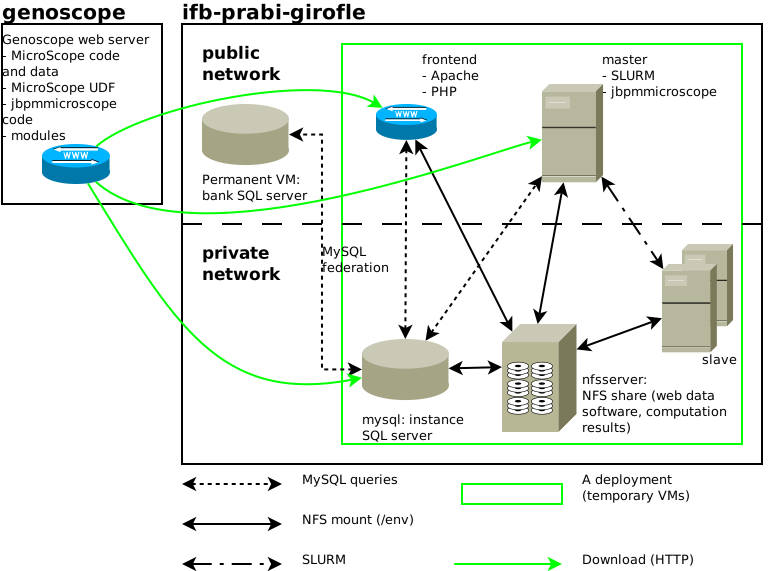
\includegraphics[width=\linewidth]{../Logical_Architecture}
    \caption{Schéma de l'architecture de MicroCloud.}
    \label{fig:architecture}
\end{figure}

Un des buts est de mimer ce qui est fait au Genoscope
c'est-à-dire que:
\begin{enumerate}
    \item Les différents composants (serveur web, serveur de BD) tournent sur des machines séparées.
    \item Les calculs tournent sur des machines séparées: l'architecture contient donc un cluster (basé sur SLURM).
\end{enumerate}
Une des seules différences est que le serveur \component{jbpmmicroscope} tourne
sur la machine frontale du cluster.

Il y a 2 serveurs de bases de données dans MicroCloud:
\begin{itemize}
    \item Un serveur MySQL installé via Docker dans la VM MySQL.
    \item Un serveur MySQL sur la VM permanente.
\end{itemize}

\section {Installation et déploiement des VM}

Le code des VM Nuvla est dans le dépôt biosphere-microcloud (\url{https://github.com/IFB-ElixirFr/biosphere-microcloud/}).
Il y a un dossier par VM et un fichier \filename{README.md} dans chaque dossier qui explique des détails.
Les principes du déploiement sont décrits sur le wiki du projet (voir la page
\href{https://intranet.genoscope.cns.fr/agc/redmine/projects/microcloud/wiki/Principes_de_fonctionnement_du_cloud_IFB}
{[[Principes de fonctionnement du cloud IFB]]}
en particulier la section
\href{https://intranet.genoscope.cns.fr/agc/redmine/projects/microcloud/wiki/Principes_de_fonctionnement_du_cloud_IFB#Utilisation-de-deacutepocircts-git-pour-le-code}
{[[Principes de fonctionnement du cloud IFB\#Utilisation-de-deacutepocircts-git-pour-le-code]]}
).

Les sections suivantes présentent quelques détails sur les VM:
\begin{itemize}
    \item frontend voir section \ref{frontend}
    \item mysql voir section \ref{mysql}
    \item VM permanente voir section \ref{VMpermanente}
    \item master et slave voir section \ref{master&slave}
    \item nfsserver voir section \ref{nfsserver}
\end{itemize}
\bigskip

\subsection {VM frontend}\label{frontend}

\todo[inline]{Ajouter une section sur les scripts côté serveur qui permettent d'installer le logiciel.}

La VM frontend permet de déployer la partie web de la plateforme MicroScope.
L'image de base est une image CentOS 7.

Le code est dans le dossier frontend (voir \url{https://github.com/IFB-ElixirFr/biosphere-microcloud/tree/master/frontend/}).
Le composant slipstream est dans le dossier frontend (voir \url{https://nuv.la/module/ifb/devzone/MicroCloud/frontend/}).
\bigskip

Lors du déploiement de la VM le code web est copié dans le répertoire \textbf{/var/www/html/} de la VM.
\bigskip

La VM frontend utilise un client mariaDB (et non pas MySQL du fait de conflits existants entre le dépôt remi-php71 installé et le dépôt IUS qui fournit le client MySQL).



\begin{mycolorbox}
    Si le message d'erreur \textbf{256} s'affiche, cela signifie simplement qu'il n'y a pas d'organisme en base.
    De ce fait, la plupart des onglets ainsi que le formulaire d'authentification sont inaccessibles.
    Ceci ne doit pas arriver si le déploiement se passe bien car on on copie les données d'un organisme.
\end{mycolorbox}

\subsection {VM mysql}\label{mysql}

Le code est dans le dossier mysql voir \url{https://github.com/IFB-ElixirFr/biosphere-microcloud/tree/master/mysql/}.
Le composant slipstream est dans le dossier mysql voir \url{https://nuv.la/module/ifb/devzone/MicroCloud/mysql/}.

L'image de base est une image CentOS 7. La VM mysql possède un serveur MySQL installé via Docker sur lequel on retrouve les bases de données pkgdb, GO\_CPD, GO\_Conf, GO\_RES, PUB\_CPD, REFSEQDB, JBPMmicroscope et PRESTATIONDB. Les tables nécessaires à l'installation de MicroScope sont également listées dans le wiki : \url{https://intranet.genoscope.cns.fr/agc/redmine/projects/microcloud/wiki/Tables_necessaires_a_installation}.
\newline

Pour se connecter à la VM mysql, il faut passer par le frontend :
\begin{lstlisting}[style=bash]
$ ssh -A centos@${IP_mysql} -J centos@${IP_frontend}
\end{lstlisting}
\bigskip

Si le serveur ne répond pas, il faut aller voir si le docker n'a pas planté (cela arrive pour des requêtes SQL trop gourmandes en RAM).
Pour relancer le docker :
\begin{lstlisting}[style=bash]
$ sudo su
$ docker ps -a
$ docker start ${ID_container}
\end{lstlisting}

\subsection {VM permanente}\label{VMpermanente}

C'est une VM OpenStack (\textbf{umr5558-microcloud.univ-lyon1.fr}) du cloud \cloudInstance{ifb-prabi-girofle} disposant de 200 Go de stockage et 8 Go de RAM (elle est actuellement sous-dimensionnée par rapport à nos besoins). La machine a été installée avec Sylvain Bonneval. L'image de base est une image Debian 9.8.

La machine permanente n'est accessible depuis l'extérieur qu'en SSH donc nous ne pouvons pas y accéder en MySQL (port 3306) depuis un autre cloud.
\newline

La procédure d'installation est dans le fichier \textbf{Installation.md} du répertoire \textbf{/root}. La VM permanente sert au stockage des données des banques. Nous avons utilisé \textbf{rsync} pour l'import des données dans le serveur MySQL.
\newline

Logiciels installés : serveur MySQL, rsync, phpMyAdmin (installé mais non configuré). 
\newline

Pour se connecter : 
\begin{lstlisting}[style=bash]
$ ssh root@134.214.33.214
\end{lstlisting}
\bigskip

Sur le serveur MySQL, il y a les schémas des bases DB et une partie des données de la base pour les tests (nous avons testés les onglets \textbf{Genome Browser}, \textbf{Identical Gene Names}) :
\begin{itemize}
    \item les bases ANTISMASHDB, CARDDB, COGDB, EGGNOGDB, ENZYMEDB, ESSDB, FIGFAMDB, INTERPRODATADB, KEGGDB, RHEADB, TAXONOMYDB, TIGRFAMDB, UNIFIREDB, UNIPROTKBDB, VIRULENCEDB, microcyc, DBWorkflow
    \item les données (en partie) de la base UNIPROTKBDB pour les tests
    \item les données de DBWORKFLOW
    \item les données de l'organisme \textit{Acinetobacter} dans la base TAXONOMYDB (taxon id 202950)
\end{itemize}

Le script \script{microscopeDBschema.py} du module MicroCloud a été utilisé pour créer les schémas.
\newline

Pour se connecter au serveur MySQL :
\begin{lstlisting}[style=bash]
$ mysql -p{MOT_DE_PASSE_SERVEUR_MYSQL_VM_PERMANENTE}
\end{lstlisting}

Les mots de passe (serveur MySQL et phpMyAdmin) sont stockés dans le répertoire \textbf{/root} de la VM.
\newline 

Pour copier les données, mieux vaut utiliser rsync et copier les données dans le répertoire \textbf{/var/lib/mysql-files/} de la VM permanente avant insertion en base.

\begin{lstlisting}[style=bash]
$ LOAD DATA INFILE '/var/lib/mysql-files/$file.DB' INTO TABLE $table;
\end{lstlisting}

\subsection{VM master et VM slave(s)} \label{master&slave}

\todo[inline]{Ajouter les notes sur jbpmmicroscope ici ? Notes sur conda et l'installation des modules ?}

Le code d'installation de ces VM est dans le dépôt de biosphere-commons : \url{https://github.com/IFB-ElixirFr/biosphere-commons}.
L'image de base est une image Ubuntu 18. Le code slipstream est basé sur les travaux de Jonathan Lorenzo et Bryan Brancotte. 

Les composants slurm master et slave ont été copiés depuis l'appliance Slurm\_Cluster\_ubuntu18 voir \url{https://nuv.la/module/ifb/devzone/jlorenzo/cluster/Slurm_Cluster_ubuntu18}.

Concernant la VM master, le code est dans le dossier master; voir
\url{https://github.com/IFB-ElixirFr/biosphere-microcloud/tree/master/master/}.
Le code du composant slipstream est dans le dossier master voir; \url{https://nuv.la/module/ifb/devzone/MicroCloud/master/}.

Pour la VM slave, voir les dossiers correspondants.\newline

Nous avons installé le moteur de workflow jBPM couplé avec un cluster slurm sur la VM master. L'ordonnancement des wokflows est ensuite géré à l'aide du cluster slurm. La VM master étant considérée comme la machine maître et les VM slaves comme noeuds de calcul.
\bigskip

Le serveur d'application Tomcat est installé (version tomcat-9.0.31 : \url{http://mirrors.ircam.fr/pub/apache/tomcat/tomcat-9/v9.0.31/bin/apache-tomcat-9.0.31.tar.gz}).
Il est utilisé comme serveur par jBPM (pour accéder à Tomcat : http://\$IP\_master).
\bigskip

Nous avons également eu besoin d'installer Pegasus-mpi-cluster (version 4.9.2 : \url{https://github.com/pegasus-isi/pegasus/archive/4.9.2.zip}) en complément de jBPM. Lors de l'installation de pegasus-mpi-cluster, la librairie libnuma a posé problème mais celle-ci n'est pas nécessaire pour les architectures non NUMA (voir \url{https://github.com/IFB-ElixirFr/biosphere-microcloud/blob/master/master/04_deployment.sh}).

\bigskip
Chaque workflow fait appel à différents modules qu'il faut installer au préalable sur la VM master. Le script \url{https://github.com/IFB-ElixirFr/biosphere-microcloud/blob/master/master/import_modules.sh} permet d'importer les archives des différents modules nécessaires au fonctionnement des workflows (WF DIRECTON principalement).
Le lancement des workflows se fait à l'aide du module bagsub lui-même lancé par jBPM. Nous avons fait quelques modifications du module bagsub afin qu'il puisse être utilisé dans l'environnement fourni par la VM master. Le script \script{import\_modules.sh} modifie le module bagsub, en supprimant l'option ulimit qui ne fonctionne pas en Dash, et, en ajoutant le paramètre MCA btl\_tcp\_if\_exclude pour exclure les interfaces réseaux docker0 et lo qui peuvent engendrer des conflits lors du lancement de jobs slurm.


\subsection{VM nfsserver} \label{nfsserver}

Le composant nfsserver a été créé en s'inspirant du travail de Stéphane Delmotte.
Il permet de fournir un dossier partagé entre les différentes VM.

L'image de base est une image CentOS 7.
Le code est dans le dossier nfsserver voir  \url{https://github.com/IFB-ElixirFr/biosphere-microcloud/tree/master/nfsserver/}.
Le composant slipstream est dans le dossier nfsserver voir
\url{https://nuv.la/module/ifb/devzone/MicroCloud/nfsserver/}.

Le répertoire \path{/var/nfsshare} du serveur NFS est monté dans le répertoire \path{/env}
des VM frontend, backend, master et slave(s).
Le répertoire \textbf{/env} se veut similaire au répertoire de même nom sur le cluster etna. 
Les fonctions permettant la création du répertoire partagé sont dans le fichier \url{https://github.com/IFB-ElixirFr/biosphere-microcloud/blob/master/lib.sh}.



\chapter{Module \micWEBdeployVer}

\todo[inline]{Ajouter une section sur les scripts côté serveur qui permettent d'installer le logiciel.}

Ce module contient les scripts utilisés pour gérer les logiciels et les données nécessaires pour déployer MicroCloud (voir~\autoref{chap:creer_nouvelle_version}).
C'est une version de développement basée sur \module[1.0]{micWEBdeploy}.

Il est constitué des scripts suivants:
\begin{description}
	\item[\script{microscopeRelease.py}]: copie le code du web, compile le code JavaScript (avec \script{microscopeCompileJS.sh}), copie les schémas de certaines bases et les données minimales de certaines bases.
	\item[\script{microscopeCopyOid.py}]: permet de copier les données de l'organisme \textit{Acinetobacter baylyi} (O\_id=31)
	\item[\script{createModulesTarball.py}]: créé les archives des modules à importer dans MicroCloud.
\end{description}

\section{\script{microscopeRelease.py}}

Les schémas copiés sont : pkgdb, REFSEQDB, GO\_Conf, GO\_RES, GO\_CPD, PUB\_CPD et PRESTATIONDB.
\newline

Les données copiées sont : pkgdb (tables : Maintenance, Country, Amiga\_Params,
Annotator pour A\_name='guest', Sequence\_Checkpoint\_Desc et Sid\_Config), GO\_RES (tables : ORGCLUST\_clustering\_param et ORGCLUST\_distance\_param.
) et GO\_Conf (prendre les données de toutes les tables). Voir page wiki : \url{https://intranet.genoscope.cns.fr/agc/redmine/projects/microcloud/wiki/Tables_necessaires_a_installation}


\section{\script{createModulesTarball.py}}

Créé les liens symboliques dans \path{/env/cns/wwwext/html/agc/ftp/MicroCloud}.
Créé le fichier \path{modules.txt} dans \path{/env/cns/wwwext/html/agc/ftp/MicroCloud}.
\newline
Puis, la VM master importe les modules listés dans modules.txt (voir \url{https://github.com/IFB-ElixirFr/biosphere-microcloud/blob/master/master/import_modules.sh}).

\begin{lstlisting}[style=bash]
createModulesTarball.py --modules_list bagsub-2.4.3 AGCScriptToolMic-2.0 micGenome-7.0.0 micJBPMwrapper-3.10.8 micPrestation-2.0 micDirecton-1.0
\end{lstlisting}

\section{\script{microscopeCopyOid.py}}

\begin{mycolorbox}
	Pour le moment seules les données concernant l'O\_id 31 peuvent être récupérées avec le script microscopeCopyOid.py car certains organismes ont besoin de tables spécifiques de la base GO\_SPE (typiquement la table acineto\_KO pour Acinetobacter baylyi).
\end{mycolorbox}

\begin{lstlisting}[style=bash]
microscopeCopyOid.py --oid 31 --output /env/cns/wwwext/html/agc/ftp/MicroCloud/microscope_31.tar.gz
\end{lstlisting}

\section{\script{microscopeCreateDBschemas.py}}
A permis de générer les .sql utilisés pour créer les schémas des bases de données dans la VM permanente.

\begin{lstlisting}[style=bash]
microscopeCreateDBschemas.py --output /env/cns/wwwext/html/agc/ftp/MicroCloud/DBschemas.tar.gz
\end{lstlisting}

\section{\script{taxonomyDBCopyTaxId.py}}
Permet de copier les données de la base TAXONOMYDB pour un tax\_id donné.

\begin{lstlisting}[style=bash]
taxonomyDBCopyTaxId.py --tax_id 202950 --output /env/cns/wwwext/html/agc/ftp/MicroCloud/taxonomyDBCopyTaxId.tar.gz
\end{lstlisting}

\section{Les scripts côtés server}

Ils sont accessibles à l'adresse : \url{https://github.com/IFB-ElixirFr/biosphere-microcloud/tree/master/frontend} et sont exécutés sur la VM frontend.
\begin{description}
	\item[\script{install\_microscope.sh}] :  ce script contient les commandes SQL permettant de créer les schémas des bases de données et d'insérer les données dans le serveur de la VM mysql. Il utilise les fichiers générés par le script microscopeRelease.py.
	\item[\script{create\_federated\_links.sh}] : ce script permet de créer des liens federated entre le serveur de la VM mysql et le serveur de la VM permanente.
	\item[\script{import\_Oid.sh}] : ce script sert à insérer les données récupérées à l'aide du script microscopeCopyOid.py. Il permet de copier les web\_data dans le répertoire approprié.
\end{description}



\section{Informations logiciels}

\subsection{Tomcat}
Version de Tomcat installée : tomcat-9.0.31 \url {http://mirrors.ircam.fr/pub/apache/tomcat/tomcat-9/v9.0.31/bin/apache-tomcat-9.0.31.tar.gz}

\subsection{Pegasus-mpi-cluster}
Liste des release : \url{https://github.com/pegasus-isi/pegasus/releases}.
C'est la version 4.9.2 \url {https://github.com/pegasus-isi/pegasus/archive/4.9.2.zip} qui est installée dans MicroCloud (version 4.6.2 dans MicroScope).
La librairie libnuma pose problème lors de l'installation de pegasus-mpi-cluster mais celle-ci n'est pas nécessaire pour les architectures non NUMA (cf. master : \url{https://github.com/IFB-ElixirFr/biosphere-microcloud/blob/master/master/04_deployment.sh}).

\subsection{Bagsub}
Le script import\_modules.sh \url {https://github.com/IFB-ElixirFr/biosphere-microcloud/blob/master/master/import_modules.sh} modifie le module bagsub, en supprimant l'option ulimit qui ne fonctionne pas en Dash, et, en ajoutant le paramètre MCA btl\_tcp\_if\_exclude pour exclure les interfaces réseaux docker0 et lo qui peuvent engendrer des conflits lors du lancement de jobs slurm.

\subsection{JBPM}
Voir les documents :
\begin{itemize}
\item Bilan jBPM
 \url{https://docs.google.com/document/d/1jKhNCV0Po0t0Z1Zru7Qe2KnJA8_8yIjictccrYvGksU/edit#heading=h.7uty8jgvcw4i} 
\item Installation jBPM \url{https://docs.google.com/document/d/1kCW1xjsifGyQiZYWtgj2ul9jX6FdCF7xknBirS-gB5k/edit}{}.
\end{itemize}

\subsection{BioMAJ}

Nous avons implémenté un certain nombre de chose dans BioMAJ, notamment dans le cadre du projet PANGBANK :
\begin{itemize}
    \item Utilisation des hardlinks lors de la mise à jour d'une banque
    \item Ajout d'options SSL
    \item Refactoring des downloaders
    \item Retry plus intelligent lors des téléchargements
\end{itemize}
\bigskip

Actuellement nous n'avons pas suffisamment de place pour installer BioMaJ sur la VM permanente.
Certaines banques sont déjà accessibles depuis les autres cloud mais pas depuis prabi-girofle (qui nous donne accès à la VM permanente).

\subsection{Conda}
À l'heure actuelle, \textbf{conda} ne me semble pas totalement adapté à nos besoins.
En effet, installer un environnement par WF est lourd (plusieurs centaines de Mo/environnement); l'autre possibilité est d'installer un environnement pour chaque groupe d'outils compatibles mais on doit gérer ça manuellement.


\end{document}
